% Options for packages loaded elsewhere
\PassOptionsToPackage{unicode}{hyperref}
\PassOptionsToPackage{hyphens}{url}
%
\documentclass[
]{article}
\usepackage{amsmath,amssymb}
\usepackage{iftex}
\ifPDFTeX
  \usepackage[T1]{fontenc}
  \usepackage[utf8]{inputenc}
  \usepackage{textcomp} % provide euro and other symbols
\else % if luatex or xetex
  \usepackage{unicode-math} % this also loads fontspec
  \defaultfontfeatures{Scale=MatchLowercase}
  \defaultfontfeatures[\rmfamily]{Ligatures=TeX,Scale=1}
\fi
\usepackage{lmodern}
\ifPDFTeX\else
  % xetex/luatex font selection
\fi
% Use upquote if available, for straight quotes in verbatim environments
\IfFileExists{upquote.sty}{\usepackage{upquote}}{}
\IfFileExists{microtype.sty}{% use microtype if available
  \usepackage[]{microtype}
  \UseMicrotypeSet[protrusion]{basicmath} % disable protrusion for tt fonts
}{}
\makeatletter
\@ifundefined{KOMAClassName}{% if non-KOMA class
  \IfFileExists{parskip.sty}{%
    \usepackage{parskip}
  }{% else
    \setlength{\parindent}{0pt}
    \setlength{\parskip}{6pt plus 2pt minus 1pt}}
}{% if KOMA class
  \KOMAoptions{parskip=half}}
\makeatother
\usepackage{xcolor}
\usepackage[margin=1in]{geometry}
\usepackage{color}
\usepackage{fancyvrb}
\newcommand{\VerbBar}{|}
\newcommand{\VERB}{\Verb[commandchars=\\\{\}]}
\DefineVerbatimEnvironment{Highlighting}{Verbatim}{commandchars=\\\{\}}
% Add ',fontsize=\small' for more characters per line
\usepackage{framed}
\definecolor{shadecolor}{RGB}{248,248,248}
\newenvironment{Shaded}{\begin{snugshade}}{\end{snugshade}}
\newcommand{\AlertTok}[1]{\textcolor[rgb]{0.94,0.16,0.16}{#1}}
\newcommand{\AnnotationTok}[1]{\textcolor[rgb]{0.56,0.35,0.01}{\textbf{\textit{#1}}}}
\newcommand{\AttributeTok}[1]{\textcolor[rgb]{0.13,0.29,0.53}{#1}}
\newcommand{\BaseNTok}[1]{\textcolor[rgb]{0.00,0.00,0.81}{#1}}
\newcommand{\BuiltInTok}[1]{#1}
\newcommand{\CharTok}[1]{\textcolor[rgb]{0.31,0.60,0.02}{#1}}
\newcommand{\CommentTok}[1]{\textcolor[rgb]{0.56,0.35,0.01}{\textit{#1}}}
\newcommand{\CommentVarTok}[1]{\textcolor[rgb]{0.56,0.35,0.01}{\textbf{\textit{#1}}}}
\newcommand{\ConstantTok}[1]{\textcolor[rgb]{0.56,0.35,0.01}{#1}}
\newcommand{\ControlFlowTok}[1]{\textcolor[rgb]{0.13,0.29,0.53}{\textbf{#1}}}
\newcommand{\DataTypeTok}[1]{\textcolor[rgb]{0.13,0.29,0.53}{#1}}
\newcommand{\DecValTok}[1]{\textcolor[rgb]{0.00,0.00,0.81}{#1}}
\newcommand{\DocumentationTok}[1]{\textcolor[rgb]{0.56,0.35,0.01}{\textbf{\textit{#1}}}}
\newcommand{\ErrorTok}[1]{\textcolor[rgb]{0.64,0.00,0.00}{\textbf{#1}}}
\newcommand{\ExtensionTok}[1]{#1}
\newcommand{\FloatTok}[1]{\textcolor[rgb]{0.00,0.00,0.81}{#1}}
\newcommand{\FunctionTok}[1]{\textcolor[rgb]{0.13,0.29,0.53}{\textbf{#1}}}
\newcommand{\ImportTok}[1]{#1}
\newcommand{\InformationTok}[1]{\textcolor[rgb]{0.56,0.35,0.01}{\textbf{\textit{#1}}}}
\newcommand{\KeywordTok}[1]{\textcolor[rgb]{0.13,0.29,0.53}{\textbf{#1}}}
\newcommand{\NormalTok}[1]{#1}
\newcommand{\OperatorTok}[1]{\textcolor[rgb]{0.81,0.36,0.00}{\textbf{#1}}}
\newcommand{\OtherTok}[1]{\textcolor[rgb]{0.56,0.35,0.01}{#1}}
\newcommand{\PreprocessorTok}[1]{\textcolor[rgb]{0.56,0.35,0.01}{\textit{#1}}}
\newcommand{\RegionMarkerTok}[1]{#1}
\newcommand{\SpecialCharTok}[1]{\textcolor[rgb]{0.81,0.36,0.00}{\textbf{#1}}}
\newcommand{\SpecialStringTok}[1]{\textcolor[rgb]{0.31,0.60,0.02}{#1}}
\newcommand{\StringTok}[1]{\textcolor[rgb]{0.31,0.60,0.02}{#1}}
\newcommand{\VariableTok}[1]{\textcolor[rgb]{0.00,0.00,0.00}{#1}}
\newcommand{\VerbatimStringTok}[1]{\textcolor[rgb]{0.31,0.60,0.02}{#1}}
\newcommand{\WarningTok}[1]{\textcolor[rgb]{0.56,0.35,0.01}{\textbf{\textit{#1}}}}
\usepackage{graphicx}
\makeatletter
\newsavebox\pandoc@box
\newcommand*\pandocbounded[1]{% scales image to fit in text height/width
  \sbox\pandoc@box{#1}%
  \Gscale@div\@tempa{\textheight}{\dimexpr\ht\pandoc@box+\dp\pandoc@box\relax}%
  \Gscale@div\@tempb{\linewidth}{\wd\pandoc@box}%
  \ifdim\@tempb\p@<\@tempa\p@\let\@tempa\@tempb\fi% select the smaller of both
  \ifdim\@tempa\p@<\p@\scalebox{\@tempa}{\usebox\pandoc@box}%
  \else\usebox{\pandoc@box}%
  \fi%
}
% Set default figure placement to htbp
\def\fps@figure{htbp}
\makeatother
\setlength{\emergencystretch}{3em} % prevent overfull lines
\providecommand{\tightlist}{%
  \setlength{\itemsep}{0pt}\setlength{\parskip}{0pt}}
\setcounter{secnumdepth}{-\maxdimen} % remove section numbering
\usepackage{bookmark}
\IfFileExists{xurl.sty}{\usepackage{xurl}}{} % add URL line breaks if available
\urlstyle{same}
\hypersetup{
  pdftitle={Survival driven deconvolution (deSurv) reveals clinically relevant tumor and stromal gene signatures},
  hidelinks,
  pdfcreator={LaTeX via pandoc}}

\title{Survival driven deconvolution (deSurv) reveals clinically
relevant tumor and stromal gene signatures}
\author{}
\date{\vspace{-2.5em}}

\begin{document}
\maketitle

Molecular subtyping has become a cornerstone of precision oncology,
enabling the stratification of cancer patients based on distinct gene
expression patterns {[}Kandoth et al., 2013; Hoadley et al., 2018{]}.
This stratification informs prognosis, guides therapeutic decisions, and
enhances our understanding of tumor biology.

Nonnegative matrix factorization (NMF), first introduced by Lee and
Seung for image decomposition {[}Lee \& Seung, 1999{]}, has become a
widely used technique for dimensionality reduction and feature learning.
Unlike other matrix factorization approaches, the nonnegativity
constraint in NMF yields an additive, parts-based representation that
facilitates interpretability of latent factors. These properties have
motivated extensive methodological development, leading to extensions
that incorporate domain knowledge, structural constraints, or
supervision. Examples include sparsity-regularized formulations
{[}Hoyer, 2004{]}, graph-regularized NMF {[}Cai et al., 2008{]}, and
more recent supervised formulations such as NMFProfiler for multi-omics
integration and clinical stratification {[}Mercadié et al., 2025{]}, as
well as Bayesian multi-study NMF frameworks for mutational signatures
{[}Grabski et al., 2025{]}. Collectively, these frameworks highlight the
flexibility of NMF as a foundation for problem-specific decompositions.

High-throughput cancer transcriptomic datasets pose unique challenges
for matrix factorization: they are high-dimensional, reflect mixtures of
tumor and stromal populations, and are increasingly paired with censored
survival outcomes. Standard applications of NMF in this domain typically
follow a two-stage procedure---first identifying latent factors in an
unsupervised manner, then testing their association with overall
survival {[}Brunet et al., 2004; Bailey et al., 2016{]}. This
retrospective strategy can uncover biologically meaningful patterns, but
it does not optimize the decomposition with respect to patient outcomes,
often yielding factors dominated by non-prognostic variation such as
tumor purity, stromal admixture, or batch effects {[}Aran et al., 2017;
Thorsson et al., 2018{]}. Although supervised and discriminant variants
of NMF have been explored {[}Tran et al., 2024{]}, and some recent works
have coupled factorization with survival analysis (e.g., Learning
Individual Survival Models from PanCancer Whole Transcriptomes {[}Kumar
et al., 2023{]}; CoxNTF {[}Fogel et al., 2025{]}), these approaches
either treat survival as a downstream predictor or rely on tensor
factorizations not tailored to high-dimensional gene expression data.

To address this gap, we introduce deSurv, a survival-driven
deconvolution framework that integrates NMF with the Cox proportional
hazards model {[}Cox, 1972{]}. deSurv directly incorporates survival
information during factorization, producing interpretable, prognostic
components while providing principled model selection criteria and
regularization for high-dimensional stability {[}Tibshirani, 1997{]}.
Implemented in a scalable pipeline for large cohorts, deSurv improves
survival prediction relative to conventional unsupervised NMF while
retaining interpretability. These results establish deSurv as a general
framework for outcome-driven molecular subtyping across cancer types.

\section*{Results}\label{results}
\addcontentsline{toc}{section}{Results}

\begin{Shaded}
\begin{Highlighting}[]
\FunctionTok{library}\NormalTok{(targets)}
\FunctionTok{library}\NormalTok{(dplyr)}
\FunctionTok{library}\NormalTok{(ggplot2)}
\NormalTok{PKG\_VERSION        }\OtherTok{=}\NormalTok{ utils}\SpecialCharTok{::}\FunctionTok{packageDescription}\NormalTok{(}\StringTok{"coxNMF"}\NormalTok{, }\AttributeTok{fields =} \StringTok{"RemoteRef"}\NormalTok{)}
\NormalTok{GIT\_BRANCH         }\OtherTok{=}\NormalTok{ gert}\SpecialCharTok{::}\FunctionTok{git\_branch}\NormalTok{()}
\NormalTok{store}\OtherTok{=}\FunctionTok{paste0}\NormalTok{(}\StringTok{"store\_PKG\_VERSION="}\NormalTok{,PKG\_VERSION,}\StringTok{"\_GIT\_BRANCH="}\NormalTok{,GIT\_BRANCH)}
\FunctionTok{tar\_config\_set}\NormalTok{(}\AttributeTok{store=}\NormalTok{store)}
\end{Highlighting}
\end{Shaded}

\subsection{The NMF--Cox framework provides an end-to-end workflow for
prognostic
modeling}\label{the-nmfcox-framework-provides-an-end-to-end-workflow-for-prognostic-modeling}

We developed an integrated framework that combines nonnegative matrix
factorization (NMF) with Cox proportional hazards regression to identify
latent gene expression factors associated with survival. As illustrated
in Figure 1, the workflow begins with preprocessing and normalization of
RNA-seq data, followed by NMF decomposition into patient factor loadings
(\(W\)) and gene weightings (\(H\)). A Cox model is then fit using
projected covariates derived from W. The framework incorporates a
balancing parameter \(\alpha\) to control the relative influence of
reconstruction error versus survival likelihood. Model selection is
performed via cross-validation across k, penalty parameters, and
\(\alpha\), with downstream evaluation focusing on both predictive
performance and biological interpretability.

\begin{Shaded}
\begin{Highlighting}[]
\NormalTok{knitr}\SpecialCharTok{::}\FunctionTok{include\_graphics}\NormalTok{(}\StringTok{"../figures/model\_schematic\_with\_validation.png"}\NormalTok{)}
\end{Highlighting}
\end{Shaded}

\begin{figure}
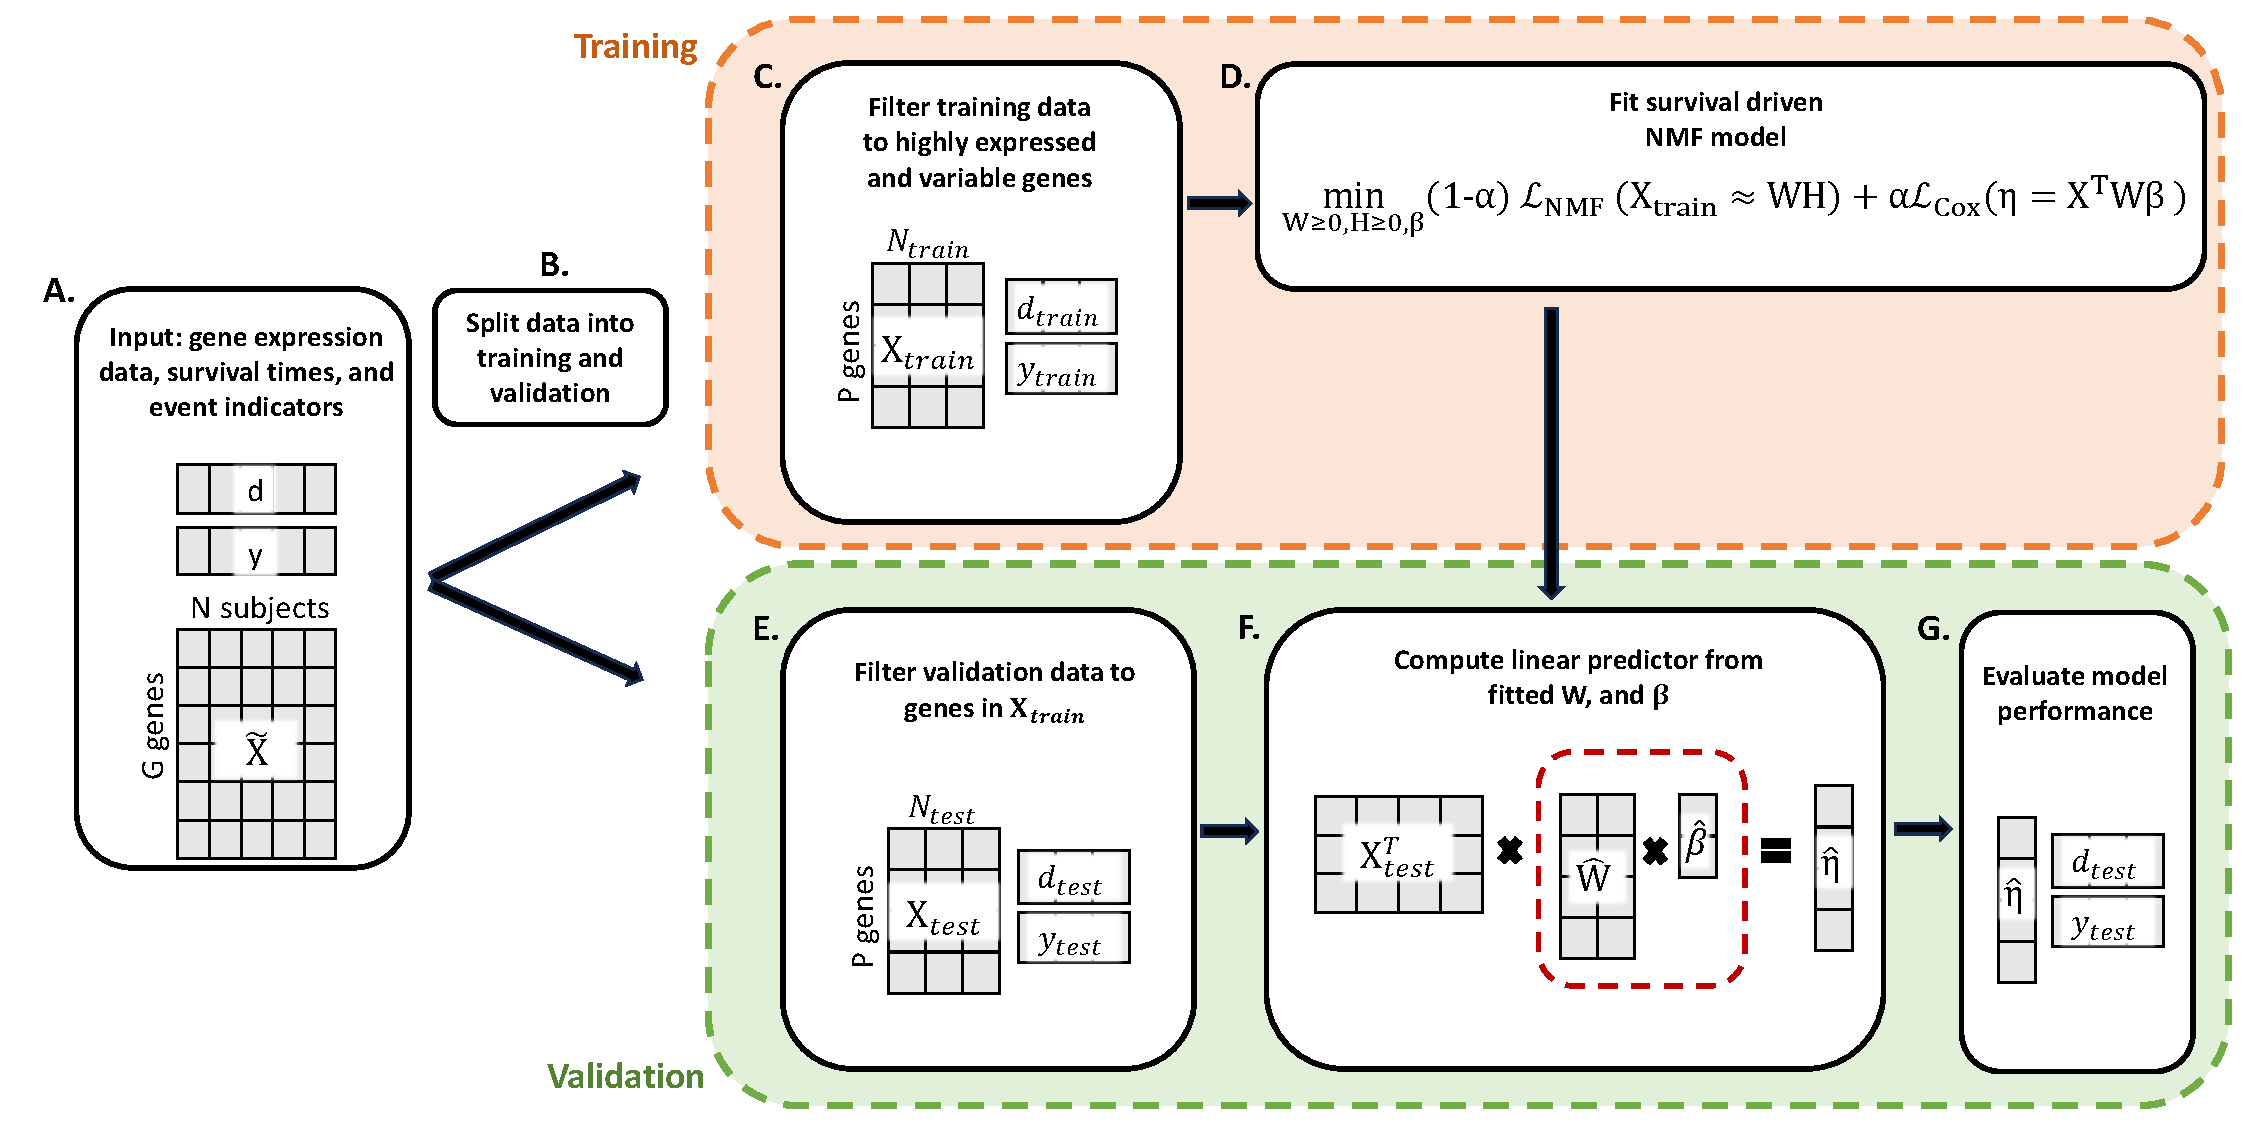
\includegraphics[width=0.8\linewidth]{../figures/model_schematic_with_validation} \caption{DeSurv overview}\label{fig:fig-schema}
\end{figure}

\subsection{The NMF--Cox model shows consistent convergence and
stability across
restarts}\label{the-nmfcox-model-shows-consistent-convergence-and-stability-across-restarts}

Across datasets and initialization schemes, the NMF--Cox algorithm
consistently converged to numerically stable solutions within the
designated iteration budget. Warm-start strategies, in which solutions
at \(\alpha=0\) initialized supervised runs, substantially reduced
variability across restarts and improved reproducibility. Figure 2 shows
representative loss trajectories demonstrating monotone decreases until
convergence, while Figure 3 summarizes performance variability across
restarts. Compared with naïve random initialization, warm-starts
produced tighter distributions of cross-validated C-index and partial
likelihood, confirming stability of the optimization procedure.

\subsection{Cross-validation of NMF--Cox identifies parameter settings
that balance prediction and
reconstruction}\label{cross-validation-of-nmfcox-identifies-parameter-settings-that-balance-prediction-and-reconstruction}

We evaluated performance across a grid of factor ranks (k), penalties,
and values of \(\alpha\). Cross-validated C-index varied modestly across
conditions, with no consistent improvement for \(\alpha>0\). Instead,
supervised extensions altered the orientation of latent factors while
maintaining comparable discrimination. Figure @ref(fig::fig-cv)A shows a
heatmap of mean C-index across k and \(\alpha\), and @ref(fig::fig-cv)B
illustrates C-index trends across \(\alpha\) stratified by rank.

\begin{Shaded}
\begin{Highlighting}[]
\FunctionTok{tar\_load\_globals}\NormalTok{()}
\FunctionTok{tar\_load}\NormalTok{(cv\_metrics)}
\NormalTok{mets\_test}\OtherTok{=}\NormalTok{cv\_metrics}\SpecialCharTok{$}\NormalTok{mets\_test}
\NormalTok{avg\_init }\OtherTok{=}\NormalTok{ mets\_test }\SpecialCharTok{\%\textgreater{}\%} \FunctionTok{group\_by}\NormalTok{(k,fold,alpha,lambda,eta,lambdaW) }\SpecialCharTok{\%\textgreater{}\%}
  \FunctionTok{summarize}\NormalTok{(}\AttributeTok{c\_mean\_f =} \FunctionTok{mean}\NormalTok{(c), }\AttributeTok{pl\_mean\_f=}\FunctionTok{mean}\NormalTok{(sloss))}\SpecialCharTok{\%\textgreater{}\%}
  \FunctionTok{ungroup}\NormalTok{()}
\end{Highlighting}
\end{Shaded}

\begin{verbatim}
## `summarise()` has grouped output by 'k', 'fold', 'alpha', 'lambda', 'eta'. You can override using
## the `.groups` argument.
\end{verbatim}

\begin{Shaded}
\begin{Highlighting}[]
\NormalTok{avg\_fold }\OtherTok{=}\NormalTok{ avg\_init }\SpecialCharTok{\%\textgreater{}\%} \FunctionTok{group\_by}\NormalTok{(k,alpha,lambda,eta,lambdaW) }\SpecialCharTok{\%\textgreater{}\%}
  \FunctionTok{summarize}\NormalTok{(}\AttributeTok{c\_mean =} \FunctionTok{mean}\NormalTok{(c\_mean\_f), }\AttributeTok{pl\_mean =} \FunctionTok{mean}\NormalTok{(pl\_mean\_f),}
            \AttributeTok{c\_sd =} \FunctionTok{sqrt}\NormalTok{(}\FunctionTok{sum}\NormalTok{((c\_mean\_f}\SpecialCharTok{{-}}\NormalTok{c\_mean)}\SpecialCharTok{\^{}}\DecValTok{2}\NormalTok{)}\SpecialCharTok{/}\NormalTok{(NFOLD}\SpecialCharTok{*}\NormalTok{(NFOLD}\DecValTok{{-}1}\NormalTok{))), }
            \AttributeTok{pl\_sd =} \FunctionTok{sqrt}\NormalTok{(}\FunctionTok{sum}\NormalTok{((pl\_mean\_f}\SpecialCharTok{{-}}\NormalTok{pl\_mean)}\SpecialCharTok{\^{}}\DecValTok{2}\NormalTok{)}\SpecialCharTok{/}\NormalTok{(NFOLD}\SpecialCharTok{*}\NormalTok{(NFOLD}\DecValTok{{-}1}\NormalTok{))))}\SpecialCharTok{\%\textgreater{}\%}
  \FunctionTok{ungroup}\NormalTok{()}
\end{Highlighting}
\end{Shaded}

\begin{verbatim}
## `summarise()` has grouped output by 'k', 'alpha', 'lambda', 'eta'. You can override using the
## `.groups` argument.
\end{verbatim}

\begin{Shaded}
\begin{Highlighting}[]
\NormalTok{avg\_fold\_fixed\_lambda }\OtherTok{=}\NormalTok{ avg\_fold }\SpecialCharTok{\%\textgreater{}\%} \FunctionTok{filter}\NormalTok{(lambda}\SpecialCharTok{==}\DecValTok{10}\NormalTok{)}

\NormalTok{heat }\OtherTok{=} \FunctionTok{ggplot}\NormalTok{(avg\_fold\_fixed\_lambda,}\FunctionTok{aes}\NormalTok{(}\AttributeTok{x=}\NormalTok{alpha,}\AttributeTok{y=}\NormalTok{k,}\AttributeTok{fill=}\NormalTok{c\_mean))}\SpecialCharTok{+}
  \FunctionTok{geom\_tile}\NormalTok{()}\SpecialCharTok{+}
  \FunctionTok{theme\_classic}\NormalTok{(}\AttributeTok{base\_size=}\DecValTok{12}\NormalTok{)}\SpecialCharTok{+}\FunctionTok{theme}\NormalTok{(}\AttributeTok{panel.grid =} \FunctionTok{element\_blank}\NormalTok{(),}
                                    \AttributeTok{axis.line  =} \FunctionTok{element\_blank}\NormalTok{(), }
                                    \AttributeTok{axis.text =} \FunctionTok{element\_text}\NormalTok{(}\AttributeTok{size=}\DecValTok{11}\NormalTok{))}\SpecialCharTok{+}
  \FunctionTok{scale\_y\_continuous}\NormalTok{(}\AttributeTok{expand=}\FunctionTok{c}\NormalTok{(}\DecValTok{0}\NormalTok{,}\DecValTok{0}\NormalTok{),}\AttributeTok{breaks=}\DecValTok{1}\SpecialCharTok{:}\DecValTok{12}\NormalTok{)}\SpecialCharTok{+}
  \FunctionTok{scale\_x\_continuous}\NormalTok{(}\AttributeTok{expand=}\FunctionTok{c}\NormalTok{(}\DecValTok{0}\NormalTok{,}\DecValTok{0}\NormalTok{),}\AttributeTok{breaks =} \FunctionTok{c}\NormalTok{(}\DecValTok{0}\NormalTok{,.}\DecValTok{25}\NormalTok{,.}\DecValTok{5}\NormalTok{,.}\DecValTok{75}\NormalTok{,}\DecValTok{1}\NormalTok{))}\SpecialCharTok{+}
  \FunctionTok{labs}\NormalTok{(}\AttributeTok{fill=}\StringTok{"CV C{-}index"}\NormalTok{)}\SpecialCharTok{+}
  \FunctionTok{scale\_fill\_viridis\_c}\NormalTok{(}\AttributeTok{option=}\StringTok{"magma"}\NormalTok{,}\AttributeTok{direction=}\SpecialCharTok{{-}}\DecValTok{1}\NormalTok{,}\AttributeTok{labels=}\NormalTok{scales}\SpecialCharTok{::}\FunctionTok{label\_number}\NormalTok{(}\AttributeTok{accuracy=}\FloatTok{0.01}\NormalTok{))}

\NormalTok{avg\_fold\_sub\_k }\OtherTok{=}\NormalTok{ avg\_fold\_fixed\_lambda }\SpecialCharTok{\%\textgreater{}\%} \FunctionTok{filter}\NormalTok{(k }\SpecialCharTok{\%in\%} \FunctionTok{c}\NormalTok{(}\DecValTok{4}\NormalTok{,}\DecValTok{6}\NormalTok{,}\DecValTok{8}\NormalTok{,}\DecValTok{12}\NormalTok{))}
\NormalTok{avg\_fold\_sub\_k}\SpecialCharTok{$}\NormalTok{k\_lab }\OtherTok{=} \FunctionTok{factor}\NormalTok{(avg\_fold\_sub\_k}\SpecialCharTok{$}\NormalTok{k, }\AttributeTok{labels=}\FunctionTok{paste0}\NormalTok{(}\StringTok{"k = "}\NormalTok{,}\FunctionTok{c}\NormalTok{(}\DecValTok{4}\NormalTok{,}\DecValTok{6}\NormalTok{,}\DecValTok{8}\NormalTok{,}\DecValTok{12}\NormalTok{)))}

\NormalTok{panels }\OtherTok{=} \FunctionTok{ggplot}\NormalTok{(avg\_fold\_sub\_k, }\FunctionTok{aes}\NormalTok{(}\AttributeTok{x=}\NormalTok{alpha,}\AttributeTok{y=}\NormalTok{c\_mean))}\SpecialCharTok{+}
  \FunctionTok{geom\_point}\NormalTok{()}\SpecialCharTok{+}
  \FunctionTok{geom\_line}\NormalTok{()}\SpecialCharTok{+}
  \FunctionTok{geom\_errorbar}\NormalTok{(}\FunctionTok{aes}\NormalTok{(}\AttributeTok{ymin=}\NormalTok{c\_mean}\SpecialCharTok{{-}}\NormalTok{c\_sd, }\AttributeTok{ymax =}\NormalTok{ c\_mean}\SpecialCharTok{+}\NormalTok{c\_sd))}\SpecialCharTok{+}
  \FunctionTok{theme\_linedraw}\NormalTok{(}\AttributeTok{base\_size=}\DecValTok{12}\NormalTok{)}\SpecialCharTok{+}
  \FunctionTok{theme}\NormalTok{(}\AttributeTok{strip.background =} \FunctionTok{element\_rect}\NormalTok{(}\AttributeTok{fill=}\StringTok{"white"}\NormalTok{,}\AttributeTok{color=}\ConstantTok{NA}\NormalTok{),}
        \AttributeTok{strip.text =} \FunctionTok{element\_text}\NormalTok{(}\AttributeTok{color=}\StringTok{"black"}\NormalTok{,}\AttributeTok{size=}\DecValTok{12}\NormalTok{),}
        \AttributeTok{axis.text =} \FunctionTok{element\_text}\NormalTok{(}\AttributeTok{size=}\DecValTok{11}\NormalTok{))}\SpecialCharTok{+}
  \FunctionTok{facet\_wrap}\NormalTok{(}\SpecialCharTok{\textasciitilde{}}\NormalTok{k\_lab)}\SpecialCharTok{+}
  \FunctionTok{labs}\NormalTok{(}\AttributeTok{y=}\StringTok{"CV C{-}index"}\NormalTok{)}

\NormalTok{ggpubr}\SpecialCharTok{::}\FunctionTok{ggarrange}\NormalTok{(heat,panels,}\AttributeTok{ncol=}\DecValTok{2}\NormalTok{,}\AttributeTok{nrow=}\DecValTok{1}\NormalTok{,}\AttributeTok{labels=}\FunctionTok{c}\NormalTok{(}\StringTok{"A"}\NormalTok{,}\StringTok{"B"}\NormalTok{),}\AttributeTok{widths=}\FunctionTok{c}\NormalTok{(}\DecValTok{5}\NormalTok{,}\DecValTok{4}\NormalTok{))}
\end{Highlighting}
\end{Shaded}

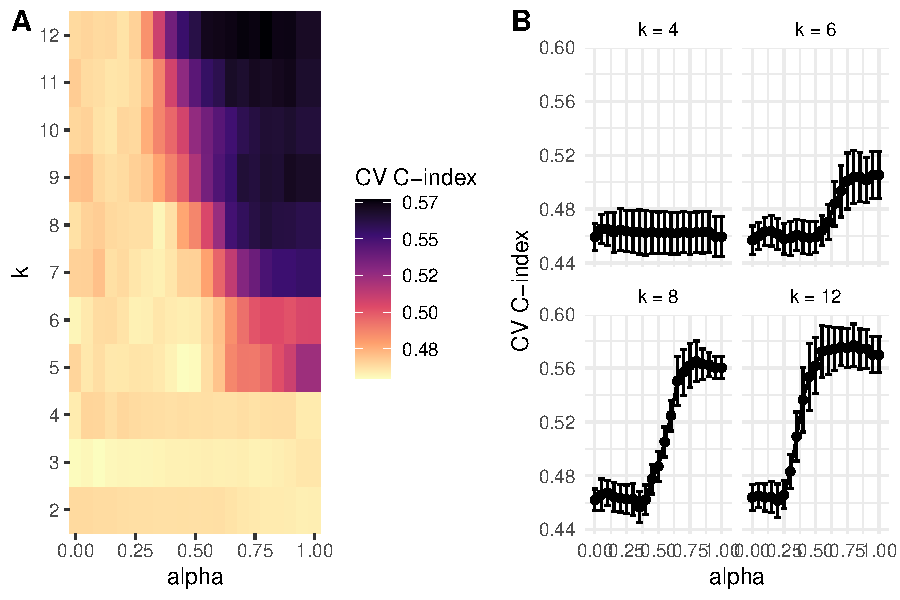
\includegraphics[width=\textwidth]{/work/users/a/y/ayoung31/DeSurv-paper/paper/paper_edits_to_pdf_files/figure-latex/fig-cv-1}

\subsection{NMF--Cox uncovers biologically interpretable latent factors
associated with clinical
outcomes}\label{nmfcox-uncovers-biologically-interpretable-latent-factors-associated-with-clinical-outcomes}

Despite limited performance gains from supervision, the latent factors
identified by NMF--Cox exhibited strong biological interpretability. The
projected covariates, \(W^TX\), aligned with known clinical and
molecular subtypes, including basal-like versus classical subgroups in
pancreatic cancer (Figure 7). Kaplan--Meier curves stratified by factor
exposures revealed significant survival differences (Figure 8),
supporting the prognostic relevance of the factors. At the gene level, W
highlighted pathway-level enrichment for immune signaling, stromal
activity, and hallmark oncogenic processes. Overlap analysis (Figure 9)
demonstrated consistency with external signatures, confirming that
NMF--Cox produces reproducible biological features.

\subsection{NMF--Cox factors generalize to independent cohorts in
external
validation}\label{nmfcox-factors-generalize-to-independent-cohorts-in-external-validation}

To assess generalizability, models trained on TCGA-PAAD and CPTAC were
applied to external cohorts including PACA, Moffitt, and Puleo. Factor
exposures in validation datasets recapitulated subgroup structures
identified in training and stratified patients into groups with distinct
survival outcomes (Figure 10). Factor correlation analyses (Figure 11)
confirmed reproducibility of core latent dimensions, particularly those
separating basal-like and classical subtypes. Predictive accuracy in
external cohorts was comparable to cross-validation results, with
simpler models (\(k\leq 5\)) showing greater reproducibility. These
findings indicate that NMF--Cox captures transferable biological signals
across studies.

\section*{Materials and methods}\label{materials-and-methods}
\addcontentsline{toc}{section}{Materials and methods}

\subsection{Joint loss function}\label{joint-loss-function}

DeSurv is constructs a joint loss function of NMF reconstruction error
and the cox partial likelihood. The contribution of each component to
the overall loss is weighted by hyperparameter \(\alpha\).

\begin{equation}
    \mathcal{L}(W,H,\beta) = (1-\alpha) \mathcal{L}(W,H)_{NMF} - \alpha \mathcal{L}(W,\beta)_{cox}
\end{equation}

\subsubsection{Reconstruction error}\label{reconstruction-error}

Let X be a matrix of \(p\) features and \(n\) subjects. Then the NMF
portion of the loss is \begin{equation}
    \mathcal{L}(W,H)_{NMF} = ||X - WH||^2_F
\end{equation} where \(W \in R^{p \times k}\) is the matrix of feature
weights and \(H \in R^{k \times n}\) is the matrix of subject weights,
where \(k\) represents the number of latent factors.

\subsubsection{Cox partial likelihood}\label{cox-partial-likelihood}

Let \(y_i = \min(T_i,C_i)\) where \(T_i\) is the event time and \(C_i\)
is the censoring time for the \(i\)th subject; let \(\delta_i\)
represent the indicator that the event time for the \(i\)th subject is
observed. Since \(W\) is not dataset dependent, we take
\(Z=X^TW \in R^{n \times k}\) to be the covariates passed to the
proportional hazards model. This can be interpreted as a transformation
of the data matrix \(X\) into the lower dimensional space. The log
partial likelihood is

\begin{equation}
    \ell(W,\beta) = \sum_{i=1}^n \delta_i \left[Z_i^T\beta - \log\left(\sum_{j=1}^n \exp \left(Z_j^T\beta\right) \mathbbm{1} (y_j \geq y_i) \right)\right]
\end{equation}

\subsection*{Update Rules}\label{update-rules}
\addcontentsline{toc}{subsection}{Update Rules}

The joint loss function in (1) is nonconvex. Algorithm (1) provides an
update alternates between updating \(W\), \(H\), and \(\beta\) until
convergence.

\begin{algorithm}
    \caption{DeSurv algorithm}\label{deSurv}

    \begin{algorithmic}[1]
        \Require $X \in \mathbb{R}_{\geq 0}^{p \times n}$, $y \in \mathbb{R}^n_{\geq 0}$, $\delta \in \mathbb{R}_{0,1}^{n}$
        \State $eps \gets \infty$
        \State $iter \gets 0$
        \State $W_{jr} \sim Unif(0,\max(X))$ for $j=1,\dots,p$ and $r=1,\dots, k$
        \State $H_{ri} \sim Unif(0, \max(X))$ for $r=1,\dots,k$ and $i=1,\dots,n$
        \While{$eps < tol$ \textbf{and} $iter < maxit$}
            \State $W \gets \argmin_{W \geq 0} \mathcal{L}(W,H,\beta)$
            \State $H \gets \argmin_{H \geq 0} \mathcal{L}(W,H,\beta)$
            \State $\beta \gets \argmin_{\beta} \mathcal{L}(W,H,\beta)$
            \State $errNew \gets \mathcal{L}(W,H,\beta)$
            \State $relErr \gets |errNew - err|/err$
            \State $err \gets errNew$
            \State $iter \gets iter + 1$
        \EndWhile
        \State \Return $W, H, \beta$
    \end{algorithmic}
\end{algorithm}

\subsubsection{H update}\label{h-update}

Since the H update does not depend on \(\beta\), a standard
multiplicative update can be used \begin{equation}
    H_{ij} = H_{ij} \frac{(W^TX)_{ij}}{(W^TWH)_{ij}}
\end{equation}

\subsubsection{\texorpdfstring{\(\beta\)
update}{\textbackslash beta update}}\label{beta-update}

Holding \(W\) fixed, the \(beta\) update for covariates \(Z\) solves the
standard convex penalized weighted least squares problem. The update as
derived in \cite{simon2011regularization} is

\begin{equation}
    \hat{\beta}_r = \frac{S(\frac{1}{n}\sum_{i=1}^n w(\Tilde{\eta})_i v_{i,r} \left[ z(\Tilde{\eta})_i - \sum_{j\ne r} v_{ij} \beta_j,\right], \lambda\xi)}{\frac{1}{n}\sum_{i=1}^n w(\Tilde{\eta})_i v_{i,r}^2 + \lambda(1-\xi)}
\end{equation}

where describe wtilde and ztilde

\subsection{Publicly Available Datasets}

To train and validate our model we used seven publicly available PDAC
datasets. RNAseq datasets were in TPM units. Each dataset was log2 + 1
transformed for variance stabilization. Additionally each dataset was
rank transformed to mitigate scale differences between datasets and
platforms. For each include sample size, citation, platform

\begin{itemize}
  \item TCGA 
  \item CPTAC
  \item Dijk
  \item Moffitt
  \item PACA array
  \item PACA seq
  \item Puleo
\end{itemize}

\subsection{Model Training}

The TCGA dataset was used for model training. The data was filtered to
the top 1000 highly expressed and variable genes. Models were trained
across a grid of hyperparameters \(\alpha \in \{0,.95\}\),
\(\lambda \in\), \(\xi \in\), \(\gamma \in\), \(\nu \in\), and
\(k = 2,\dots,15\)

\subsubsection{Hyperparameter selection}

The hyperparameters \(\alpha\), \(\lambda\), \(\xi\), \(\gamma\), and
\(\nu\) were selected to adequately balance the supervised and
unsupervised portions of the model using a metric we defined as the
c-index of the proportional hazards model divided by the reconstruction
error. The parameters were chosen to maximize this metric. Since the
reconstruction error exclusively decreases as the dimension \(k\)
increases, this metric was not adequate to choose \(k\).

Cross-validation was used to select the optimal hyperparameters. To
account for lack of uniqueness of NMF solutions, we used 50 random
initializations of W,H, and beta per fold. Validation metrics were
averaged across fold and initialization.

\subsection{Model Validation}

The remaining 7 publicly available PDAC datasets, CPTAC, Dijk, Linehan,
Moffitt, PACA microarray, PACA RNAseq, and Puleo, were used to validate
our models. The datasets were restricted to the same highly variable
genes in the TCGA dataset, and the fitted model was applied to each
dataset individually. The partial likelihood and c-index were calculated
for each dataset. Hazard ratios were reported for each factor.

\subsection{Score based approach}

In a clinical setting, it may not be feasible to sequence all of the
genes required to port the full W matrix to future test sets. For this
purpose we also propose a score based method, where only the identity of
top genes for each factor must be ported to future datasets. To
construct the scores we define Wtilde as a binary matrix\ldots{} To
predict patient outcomes in future datasets, we restrict those datasets
to these g x k genes, and compute XtWtilde as linear predictor in the
survival model.

\subsubsection{Top genes}

The top genes were extracted from each factor of W in the selected model
at each value of \(k\). A top gene was defined as \ldots{}

\showmatmethods
\showacknow
\pnasbreak

\end{document}
